\documentclass{standalone}
\usepackage{tikz}
\usetikzlibrary{arrows.meta, positioning}

\begin{document}

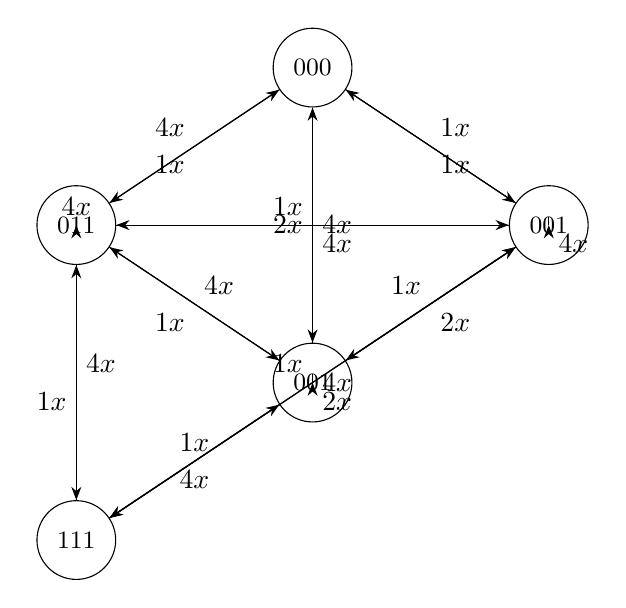
\begin{tikzpicture}[
    node/.style={circle, draw, minimum size=1cm, font=\small},
    >=Stealth,
    every edge quotes/.append style={auto, font=\footnotesize, inner sep=2pt},
    node distance=2.5cm
]

% Define nodes
\node[node] (A) at (0,0) {0 \\ 0 \\ 0};
\node[node] (B) at (-3,-2) {0 \\ 1 \\ 1};
\node[node] (C) at (3,-2) {0 \\ 0 \\ 1};
\node[node] (D) at (0,-4) {0 \\ 0 \\ 1};
\node[node] (E) at (-3,-6) {1 \\ 1 \\ 1};

% Draw edges with labels
\draw[->] (A) -- (B) node[midway, above left] {$4x$};
\draw[->] (B) -- (A) node[midway, below left] {$1x$};
\draw[->] (A) -- (C) node[midway, above right] {$1x$};
\draw[->] (C) -- (A) node[midway, below right] {$1x$};
\draw[->] (B) -- (C) node[midway, below right] {$4x$};
\draw[->] (C) -- (B) node[midway, above left] {$1x$};
\draw[->] (A) -- (D) node[midway, right] {$4x$};
\draw[->] (D) -- (A) node[midway, left] {$2x$};
\draw[->] (B) -- (D) node[midway, below left] {$1x$};
\draw[->] (D) -- (B) node[midway, above right] {$4x$};
\draw[->] (C) -- (D) node[midway, below right] {$2x$};
\draw[->] (D) -- (C) node[midway, above left] {$1x$};
\draw[->] (B) -- (E) node[midway, below left] {$1x$};
\draw[->] (E) -- (B) node[midway, above right] {$4x$};
\draw[->] (C) -- (E) node[midway, below right] {$2x$};
\draw[->] (E) -- (C) node[midway, above left] {$1x$};
\draw[->] (D) -- (E) node[midway, below] {$4x$};
\draw[->] (E) -- (D) node[midway, above] {$1x$};

% Add self-loops
\draw[->, looseness=8] (B) to[bend left] node[above] {$4x$} (B);
\draw[->, looseness=8] (C) to[bend right] node[below right] {$4x$} (C);
\draw[->, looseness=8] (D) to[bend right] node[right] {$4x$} (D);

\end{tikzpicture}

\end{document}